\section{Introduction}\label{sec:intro}

The Philippines is an archipelago of over 7,600 islands, comprising three main
regions: Luzon, the Visayas, and Mindanao. The country's mountainous terrain
and inter-island sea channels have historically restricted and directed contact
among language communities~\cite{Boquet_2017}. While linguists have documented
over 180 indigenous languages in the country~\cite{ethnologue2025},
quantitative measurements of their cross-linguistic similarities are rare.

This paper quantifies the orthographic and phonetic relationships among 16
Philippine languages, listed in~\cref{tab:ph_languages}. Traditional
Austronesian linguistics maps historical divergence using lexical comparisons,
such as cognate counts in standard word lists. We use a corpus-based method
instead. By extracting \( n \)-gram frequencies from standardized text, we
measure structural and acoustic patterns without relying on direct word
meanings. We then test these linguistic matrices against geographic distances
using a Mantel test to model how physical barriers affect language variation.

\begin{table}[h!]
    \centering
    \begin{tabular}{lc}
        \hline
        \textbf{Philippine Language} & \textbf{ISO 639} \\
        \hline
        Tagalog                      & \texttt{tgl}     \\
        Cebuano                      & \texttt{ceb}     \\
        Ilocano                      & \texttt{ilo}     \\
        Hiligaynon                   & \texttt{hil}     \\
        Bikol language~\footnotemark & \texttt{bik}     \\
        Waray-Waray                  & \texttt{war}     \\
        Kapampangan                  & \texttt{pam}     \\
        Pangasinan                   & \texttt{pag}     \\
        Adasen                       & \texttt{tiu}     \\
        Chavacano                    & \texttt{cbk}     \\
        Paranan                      & \texttt{prf}     \\
        Tausug                       & \texttt{tsg}     \\
        Romblomanon                  & \texttt{rol}     \\
        Masbatenyo                   & \texttt{msb}     \\
        Kinaray-a                    & \texttt{krj}     \\
        Yami language                & \texttt{tao}     \\
        \hline
    \end{tabular}
    \caption{Philippine languages with their ISO 639 codes}\label{tab:ph_languages}
\end{table}
\footnotetext{The code \texttt{bcl} is also used for the Bikol language.}

Philippine languages can be compared in three ways. We can compare how they are
written, how they sound, and where they are spoken. Orthographic similarity
reflects spelling convention. It can show which languages were standardised
under the same missionary, educational, or administrative influence. Phonetic
similarity reflects sound pattern and pronunciation. It tends to say more about
genetic relationships, because it is not filtered through the comparatively
recent and externally imposed layer of Latin script spelling
convention~\cite{Blust_1991}. This distinction matters for Philippine languages
in particular. Many of them adopted the Latin script during Spanish
colonization while keeping distinct, indigenous phonological systems, so two
languages can share a spelling convention for reasons that have little to do
with shared ancestry. In the same way, two languages can differ in spelling
while remaining phonetically close, which points to a shared Austronesian
history that the orthography does not show. Geography is the third point of
comparison, and it helps explain the other two. Each of the three regions of
the Philippines has its own ecological and historical conditions, and these
correspond to patterns of linguistic variation~\cite{Boquet_2017}. Much of this
diversity is attributed to the archipelago's fragmented geography, which has
restricted mobility and sustained linguistic isolation~\cite{Blust_1991}.
Mountains, rivers, and ocean channels have acted as both connectors and
separators. The \emph{barangay}, the smallest socio-political unit of
pre-colonial society, was typically sited near rivers or coasts. This location
supported trade, but it also created small pockets of linguistic autonomy,
where neighbouring islands could remain mutually unintelligible despite being
close to one another. Blust's Austronesian dispersal
hypothesis~\cite{Blust_1991} holds that a single protolanguage, introduced by
early settlers from the Asian mainland, diverged through localised adaptation
and restricted contact. Communities became isolated and accumulated their own
phonological and lexical innovations over time, and this process produced the
175 documented Philippine languages, two of which are now
extinct~\cite{ethnologue2025}. The sixteen languages studied here range from
dominant regional lingua francas to endangered local languages, and they are
examined below using all three points of comparison together.

To support this analysis, we compiled a text corpus for each language using
translated biblical texts. A biblical parallel corpus ensures semantic
alignment across the dataset; because the underlying source material is
identical, variations in \( n \)-gram frequencies reflect genuine linguistic
differences rather than topic bias.

Geographically, these 16 languages span the length of the archipelago and
beyond. Tagalog, Kapampangan, and Pangasinan are spoken in the plains of
Central Luzon. In the north, Ilocano is spoken in the coastal lowlands, Adasen
in the Cordillera interior of Abra, and Paranan on the Sierra Madre coast. The
Visayas contain a contiguous cluster of Bisayan languages—Cebuano, Hiligaynon,
Kinaray-a, and Waray-Waray—separated by narrow sea channels. Bikol, Masbatenyo,
and Romblomanon sit in the transitional zone between the Visayas and Luzon. In
the south, Tausug is spoken in the Sulu archipelago and Chavacano, a Spanish
creole, in Zamboanga. Yami, the only language outside the Philippines in this
dataset, is spoken on Orchid Island, Taiwan. As a Batanic language closely
related to Ivatan, we include it as a northern Austronesian outgroup.
\cref{fig:lingmap_out} maps the spatial distribution of these languages.

\begin{figure}[h]
    \centering
    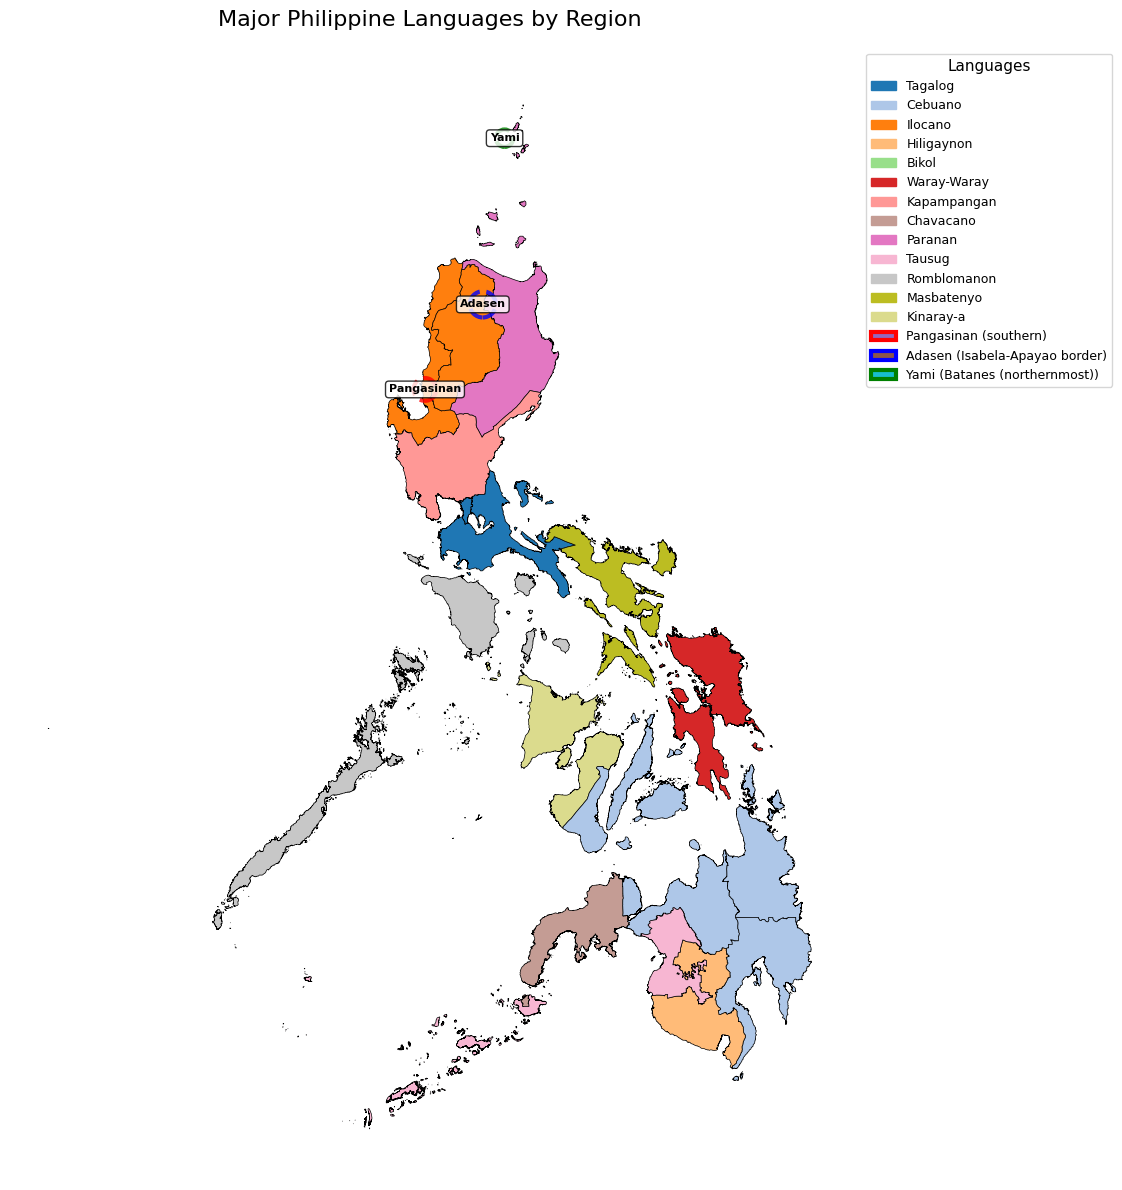
\includegraphics[width=\columnwidth]{chapters/artifacts/lingmap_out.png}
    \caption{Generated linguistic map showing the spatial distribution of the
        selected Philippine languages overlaid on topographic contours. Its
        construction is described in~\cref{sec:geo}.}
    \label{fig:lingmap_out}
\end{figure}